\chapter{Grundlagen}
\label{ch:grundlagen}
Das folgende Kapitel beschreibt elementare Grundlagen, die zum Verständnis der nachfolgenden Kapitel notwendig sind. Der
erste Abschnitt des Kapitels befasst sich mit den verwendeten Maschinen und Komponenten der Robert Bosch GmbH.

Der zweite Teil widmet sich der Künstlichen Intelligenz und den verschiedenen Untergruppen und Ausprägungen, welche in
diesem Bereich existieren. Es wird dabei unter anderem auf die Konfiguration der Produkte und Laufzeitumgebungen
eingegangen. Außerdem werden hier die Programme und Konzepzte behandelt, welche in dieser Arbeit benötigt werden.

Im letzten Teil des Kapitels folgt die Beschreibung einer Designidee bei Smartphone-Apps, allgemeine Konzepte der
Softwareentwicklung und ein Framework zum Entwickeln von Webseiten.

\section{Bosch KWE Waage}
Die Bosch KWE Serie ist ein modulares Kontrollwaagensystem, welches speziell für den Einsatz in der pharmazeutischen
Produktion entwickelt wurde. Allerdings findet es immer häufiger Verwendung im Bereich der Nahrungsmittel und
Süßigkeiten.

Um das Gewicht eines Produktes zu ermitteln, fahren die Produkte auf einem Förderband, waagerecht über die Wiegeeinheit
des Kontrollwaagensystems. Die KWE 4000 kann beispielsweise bei einer maximalen Leistung von bis zu 450 Pakete in der
Minute eine Genauigkeit von 50mg erreichen.

Das zugehörige Display zeigt Produktionsstatistiken, Trendkurven und das aktuelle Gewicht des Produktes an. Durch eigene
Konfigurationen können allerdings auch weitere Informationen auf dem Display dargestellt werden. Auf der eigenen
Herstellerseite~\cite{online_grundlagen_boschkwe} sind weitere Informationen und Ausprägungen zur aktuellen KWE-Serie
einzusehen.

Die KWE verfügt über mindestens ein Pusher-System, welches vorbeifahrende, schon gewogene Produkte vom Band schieben
kann. Dies können zum Beispiel Produkte mit falschem Gewicht oder falschen Abmaßen sein oder alle Produkte, damit sie
auf ein anderes Förderband fallen.

Die Abbildung~\ref{fig:grundlagen_boschkwe} auf Seite~\pageref{fig:grundlagen_boschkwe} zeigt eine aktuelle KWE 4000 mit
ihrem grundsätzlichen Aufbau, dem farblichen Display und einem Auffangbehälter für alle Produkte, die von dem Pusher vom
Förderband geschoben wurden.

\begin{figure}[h]
    \centering
    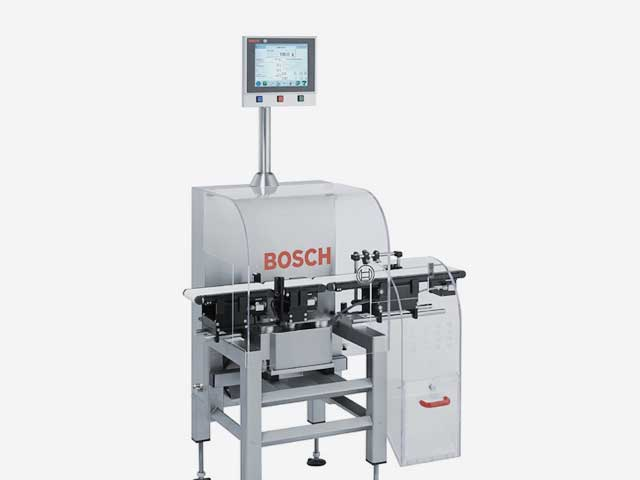
\includegraphics[scale=0.4]{images/kapitel_2/bosch_kwe.jpg}
    \caption{Abbildung einer Bosch KWE 4000}
    \label{fig:grundlagen_boschkwe}
\end{figure}

\section{Bosch Siegelmaschine}
Die Vertikale Form-, Füll- und Schließmaschine (kurz VFFS) ist für die Verpackung von  frei fließenden und losen
Lebensmittel, wie zum Beispiel Pulver, Proteine, Hähnchen sowie frische und gefrorene Produkte geeignet.

Dabei fallen die zu befüllenden Produkte vertikal aus dem oberen Bereich in den unteren Teil der Maschine. Dort baut
die Siegelmaschine zeitgleich den Behälter aus Folie zusammen, indem sie einen Schlauchbeutel formt und diesen auf
beiden äußeren Seiten verschließt. Der so geformte Endlosbeutel wird anschließend mit dem Produkt befüllt.

Der Behälter wird dann durch zwei Siegelbacken am oberen Ende verschlossen und ein Messer trennt ihn vom Rest des
Folienbandes ab. Der fertig befüllte Behälter fährt dann über ein Förderband aus der Maschine heraus und kann
weiterverarbeitet werden.

Das farbige Display dient zur Konfiguration der Maschine und kann die aktuelle Tätigkeit visualisieren. So können über
das Display alle Funktionen überwacht werden.

Die Abbildung~\ref{fig:grundlagen_boschvffs} auf Seite~\pageref{fig:grundlagen_boschvffs} zeigt eine Vertikale Form-,
Füll- und Schließmaschine mit ihrem gläsernen Befüllungsmodul und dem farbigen Display.

\begin{figure}[h]
    \centering
    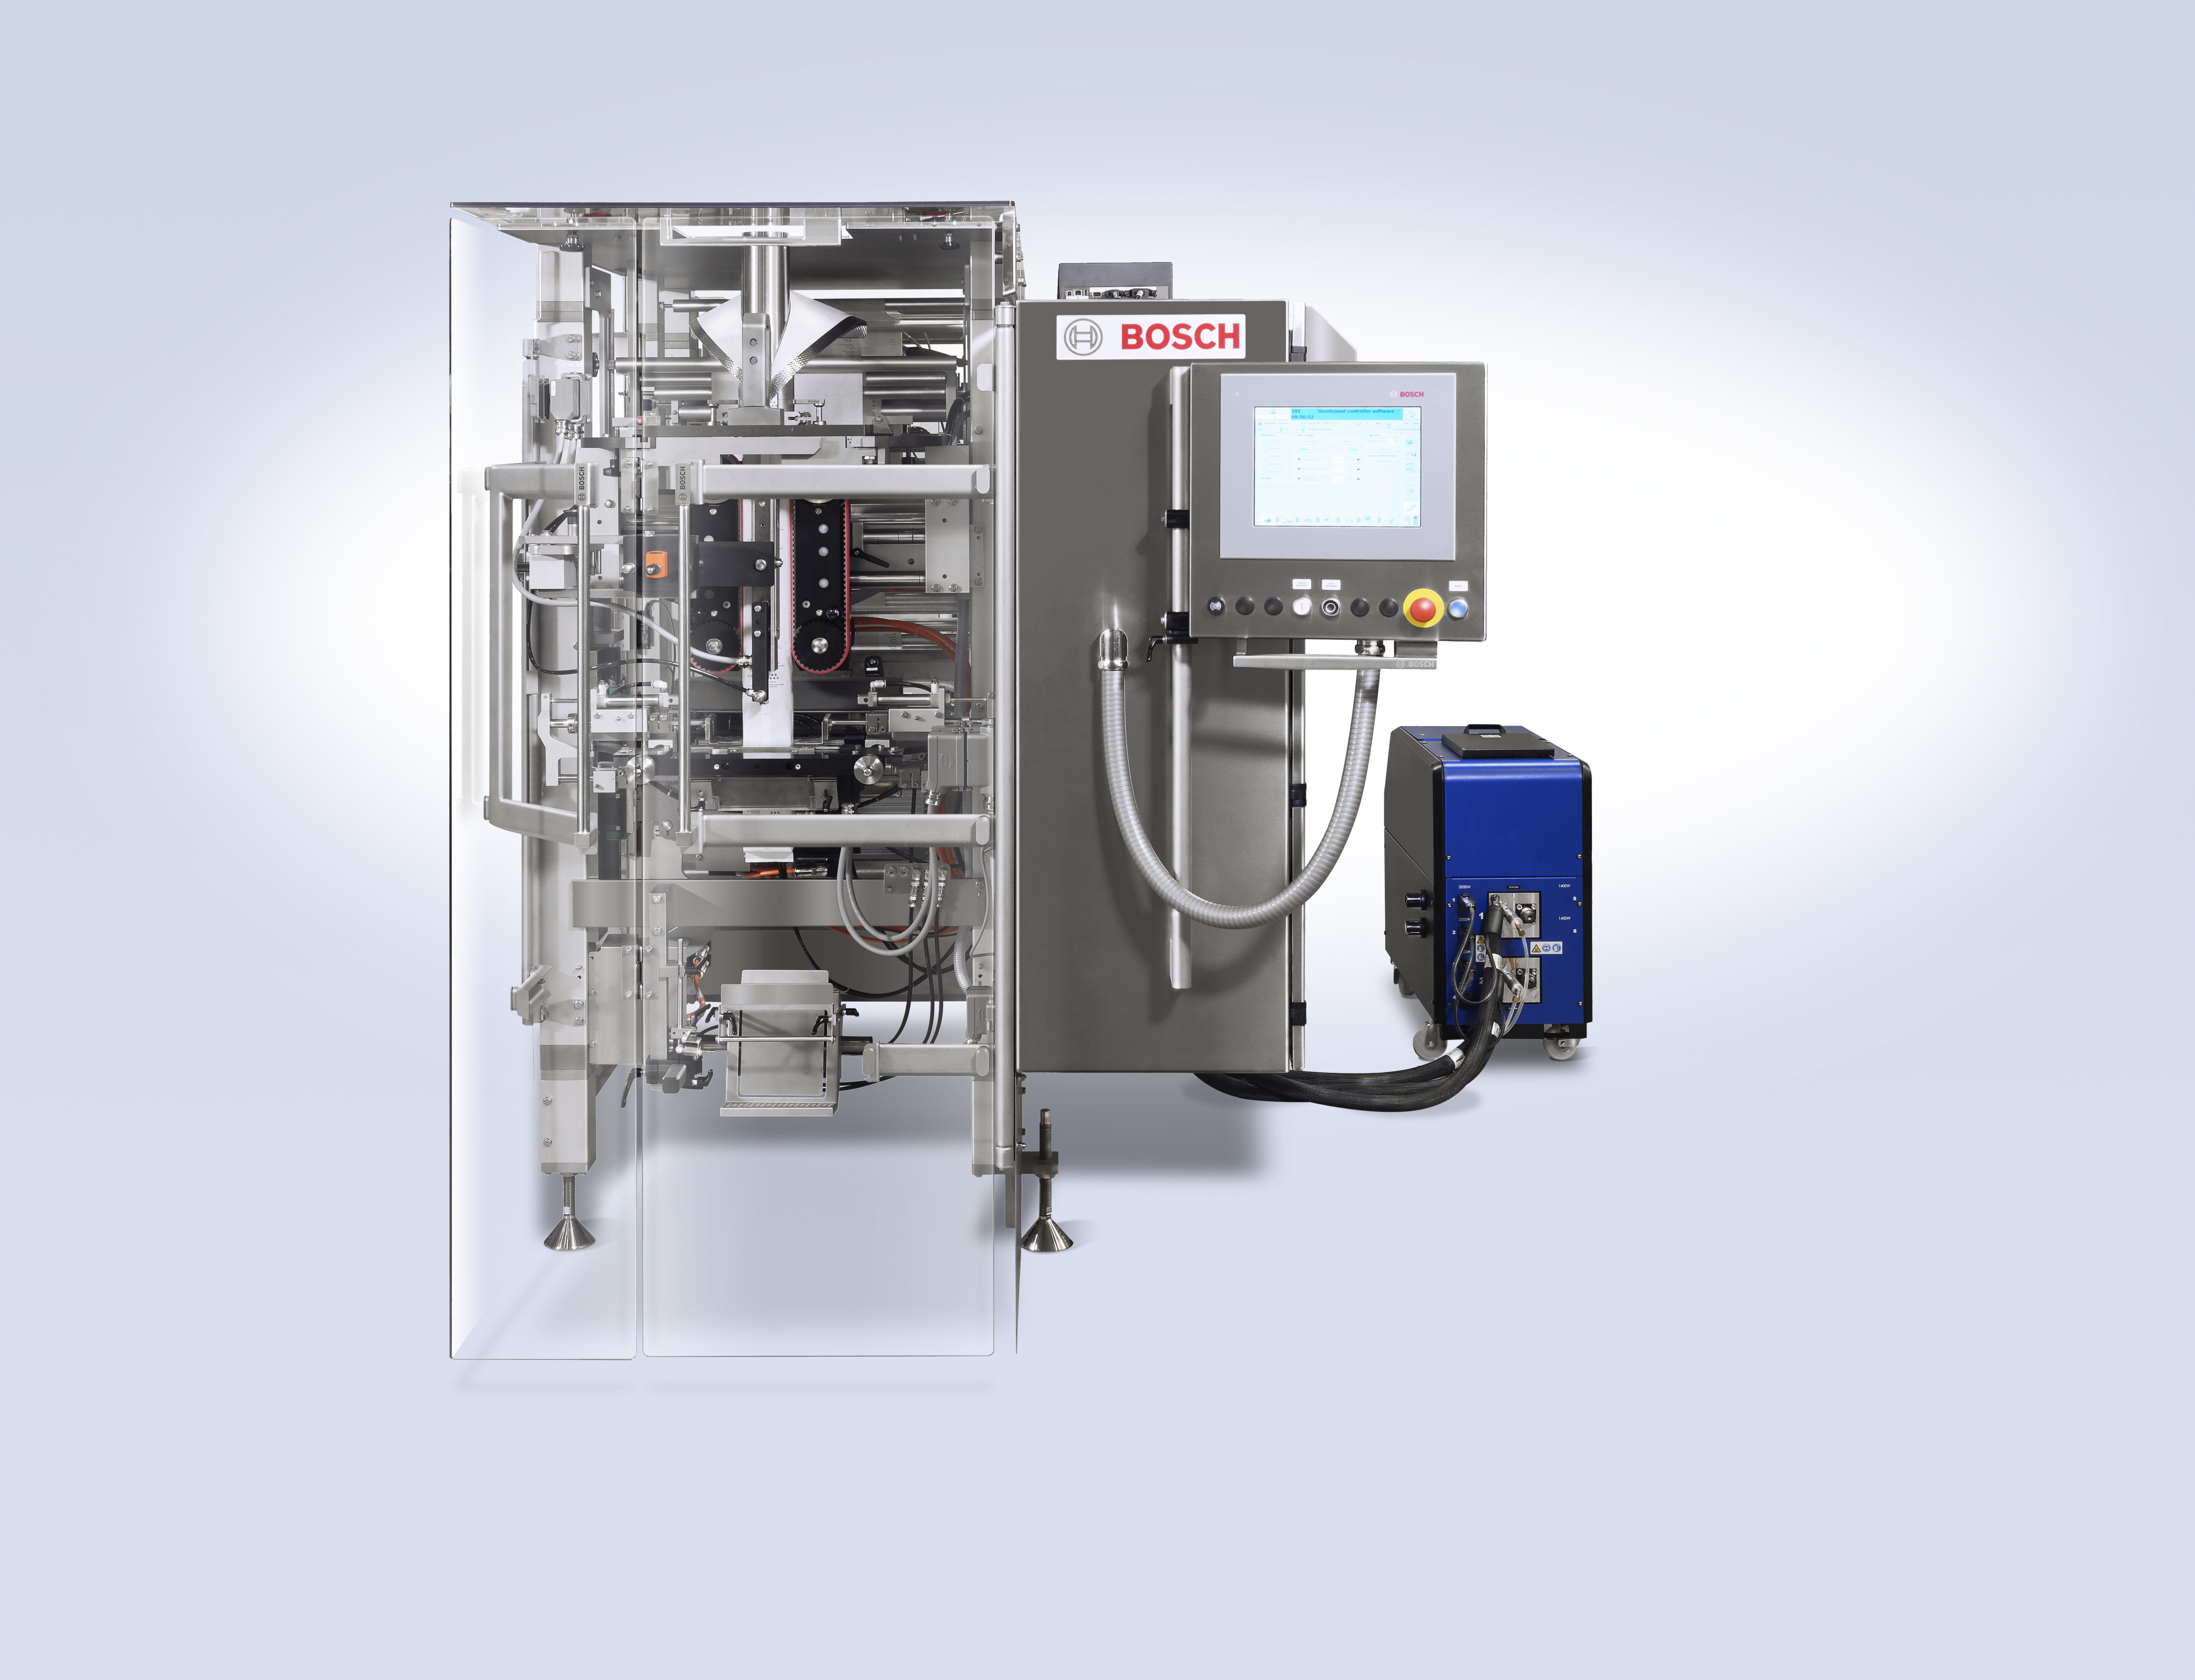
\includegraphics[scale=0.2]{images/kapitel_2/bosch_vffs.jpg}
    \caption{Abbildung einer Bosch VFFS}
    \label{fig:grundlagen_boschvffs}
\end{figure}

\section{Künstliche Intelligenz}
Künstliche Intelligenz (kurz KI) beziehungsweise Artificial Intelligence (kurz AI) ist ein Konzept für Maschinen, die
\enquote{wie Menschen denken} sollen. Dies umfasst das Lernen (die Erfassung von Informationen und Regeln für die
Verwendung der Informationen), die Schlussfolgerung (die Verwendung der Regeln, um ungefähre oder endgültige
Schlussfolgerungen zu ziehen) und die Selbstkorrektur.

Wie der KI Bundesverband e.V mitteilt, werden Maschinen in naher Zukunft noch nicht mit menschlicher Intelligenz
mithalten können. Allerdings wird sich KI auf viele Arten auf den Alltag auswirken, so der
Verein~\cite{article_grundlagen_ki}.

Die Künstliche Intelligenz kann auf verschiedene Arten kategorisiert werden. Nachfolgend zwei stellvertretende Beispiele
um eine Einordnung der verschiedenen Algorithmen zu erleichtern.

\begin{itemize}
    \item \textbf{Schwache KI} \\
    Die Schwache KI (englisch weak oder narrow AI) ist ein KI-System, das für eine bestimmte Aufgabe entwickelt und
    trainiert wird. Virtuelle persönliche Assistenten, wie der Google Assistant oder Alexa von Amazon, sind eine Form
    der schwachen KI.
    \item \textbf{Starke KI} \\
    Die starke KI (englisch strong AI) ist auch bekannt als die allgemeine künstliche Intelligenz. Sie simmuliert die
    menschlichen kognitiven Fähigkeiten und kann so noch unbekannte Aufgaben in der Zukunft lösen. Ein
    \textit{Turing Test} gibt darüber Auskunft, ob die Maschine eine starke KI besitzt.
\end{itemize}

Die Abbildung~\ref{fig:grundlagen_artificialintelligence} auf Seite~\pageref{fig:grundlagen_artificialintelligence} gibt
Auskunft über die Einteilung der Künstlichen Intelligenz in ihre Untergruppen. Dabei handelt es sich um eine eigene
Darstellung frei nach CodesOfInterest\footnote{https://codesofinterest.com/2016/11/difference-artificial-intelligence-machine-learning-deep-learning.html}.

\begin{figure}[h]
    \centering
    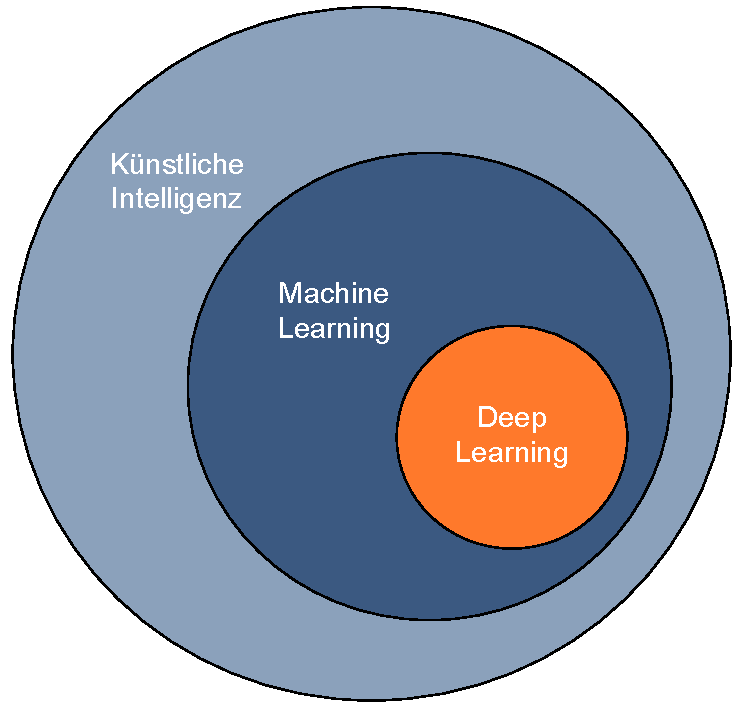
\includegraphics[scale=0.55]{images/kapitel_2/kuenstliche_intelligenz.pdf}
    \caption{Untergruppen der Künstlichen Intelligenz}
    \label{fig:grundlagen_artificialintelligence}
\end{figure}

Demnach ist \textit{Deep Learning} ein Teilbereich des \textit{Machine Learnings}, das wiederum ein Teilbereich der
\textit{Künstlichen Intelligenz} ist.

\section{Turing Test}
Der Naturwissenschaftler Alan Turing entwickelte 1950 den Turing Test. Dieser soll herausfinden, ob die Intelligenz eines
Systems der eines Menschen entspricht. Dieser Test wird regelmäßig zur Überprüfung und Einschätzung von Systemen
herangezogen.

Der Turing-Test basiert auf Konversation per Tastatur und Bildschirm, ohne jedoch Hör- und Sehkontakt zwischen den
Teilnehmern herzustellen. In dem Test sind zwei echte Personen (B und C) und die zu betestende Maschine involviert. Eine
Person (C) übernimme die Aufgabe eines Testers. Der Computer (A) und die verbleibende Person (B) bilden die kontrahenten.
Die Abbildung~\ref{fig:grundlagen_turingtest} auf Seite~\pageref{fig:grundlagen_turingtest} skizziert den Versuchsaufbau.

\begin{figure}[h]
    \centering
    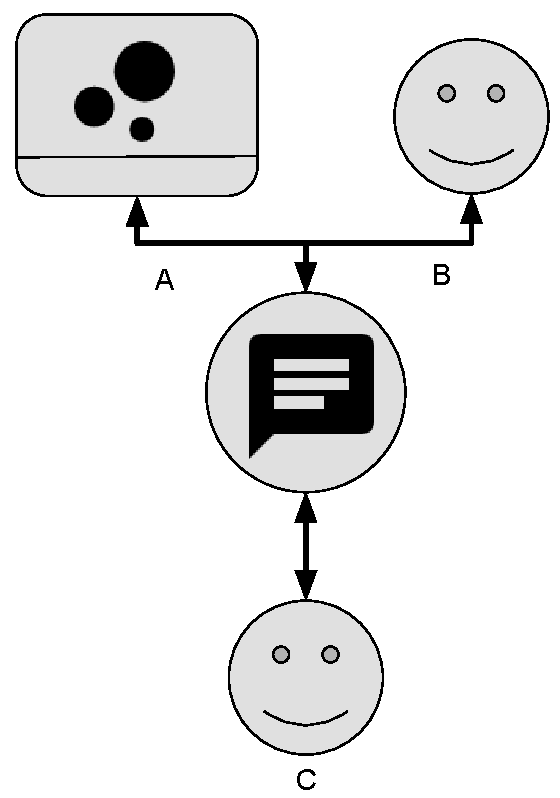
\includegraphics[scale=0.6]{images/kapitel_2/turing_test.pdf}
    \caption{Aufbau des Turing Tests}
    \label{fig:grundlagen_turingtest}
\end{figure}

Der Computer und die Person B versuchen ihren Gesprächspartner C in aufeinanderfolgenden Konversationen davon zu
überzeugen, dass sie der denkende Mensch sind. Sobald Person C nicht mehr zweifelsfrei bestätigen kann, welche
Konversation von der anderen Person und welche von der Maschine geführt wird, gilt der Test als bestanden (mehr
unter~\cite{online_grundlagen_turing}).

Jedoch ist dieser Test nicht frei von Kritik. Der Amerikanische Philosoph John Searle kritisiert zum Beispiel, dass mit
diesem Test lediglich die Funktionalität eines Systems überprüft wird, er jedoch nicht testet, ob die Maschine auch ein
Bewustsein oder eine Intentionalität hat.

Eine Maschine könnte diesen Test bestehen, wenn sie lediglich menschliches Verhalten imitiert und darauf programmiert
ist. Sie könnte den Tester so manipulieren, dass sie ihn für den echten Menschen hält.

\section{Big Data}
Mit dem Begriff Big Data wird die große Menge an strukturierten und unstrukturierten Daten, welche Unternehmen Tag für
Tag produzieren, bezeichnet.

Diese Daten können zum Beispiel aus den Bereichen des Internets und Mobilfunks, der Finanzindustrie, Energiewirtschaft,
des Gesundheitswesens und Verkehrs, sozialen Medien, Kundenkarten, Smart-Metering-Systemen und Assistenzgeräten stammen.

Einer der wichtigsten Ziele von Big Data ist es, neue Informationen oder neue Erkentnisse aus den Daten zu gewinnen.
Dazu müssen sie Analysiert werden, was erheblichen Rechenaufwand bedeutet (mehr zu Big Data
unter~\cite{book_grundlagen_bigdata}).

\section{Machine Learning}
Machine Learning ist ein Teilgebiet der Künstlichen Intelligenz und umfasst Algorithmen, mit denen Computer unter
minimalem Programmieraufwand in der Lage sind, aus Daten zu lernen.

Dabei versuchen sie anhand vorhandeneer Datenbestände und vorgegebenen Algorithmen Muster und Gesetzmäßigkeiten zu
erkennen sowie eigenständige Lösungen zu erarbeiten. Die Erkenntnisse lassen sich anschließend verallgemeinern und für
neue Problemlösungen oder für die Analyse von bisher unbekannten Daten verwenden.

Algorithmen nehmen beim maschinellen Lernen eine zentrale Rolle ein. Sie sind für das Erkennen von Mustern und das
Generieren von Lösungen verantwortlich und lassen sich in verschiedene Lernkategorien einteilen
(mehr in~\cite{book_grundlagen_machinelearning}).

\subsection{Algorithmen}
Ein Algorithmus gibt grundsätzlich eine Vorgehensweise vor, um ein Problem zu lösen (mehr zu Algorithmen
in~\cite{book_grundlagen_algorithmen}).

Machine Learning-Algorithmen ermöglichen es Computern, selbstständig zu lernen. Anstatt eine Vielzahl von Quellcode in
Form von Regeln zu programmieren, werden dafür statistische Algorithmen verwendet.

Es existieren drei Hauptkategorien für die Algorithmen im Bereich Machine Learning. Das Supervised Learning (überwachtes
Lernen), das Unsupervised Learning (unüberwachtes Lernen) und das Reinforcement Learning (bestärkendes Lernen).

Die meisten Algorithmen suchen nach Beziehungen und Zusammenhängen zwischen den Input-Daten oder zwischen den Input-
sowie den Output-Daten.

\subsubsection{Supervised Learning}
Supervised Learning, auch Random Forest genannt, basiert auf Entscheidungsbäumen (englisch Decision Trees). Es wird
sowohl für Regressionen als auch zur Klassifizierungen verwendet, da die Anforderungen an die Hardware sehr viel geringer
sind als beispielsweise bei neuronalen Netzen (mehr dazu unter~\cite{book_grundlagen_learnings}).

Entscheidungsbäume können mit einem einfachen Beispiel aus der Pflanzenwelt beschrieben werden. Das
\enquote{Hello World} des maschinellen Lernens ist die Klassifizierung von Schwertlilien (Iris). Diese werden anhand von
vier Merkmalen klassifiziert: Kelchblattlänge, Kelchblattbreite, Blütenblattlänge und Blütenblattbreite.

In Abbildung~\ref{fig:grundlagen_supervised_learning} auf Seite~\pageref{fig:grundlagen_supervised_learning} ist ein
Ausschnitt des Entscheidungsbaumes zur klassifizierung von Schwertlilien zu sehen.

\begin{figure}[h]
    \centering
    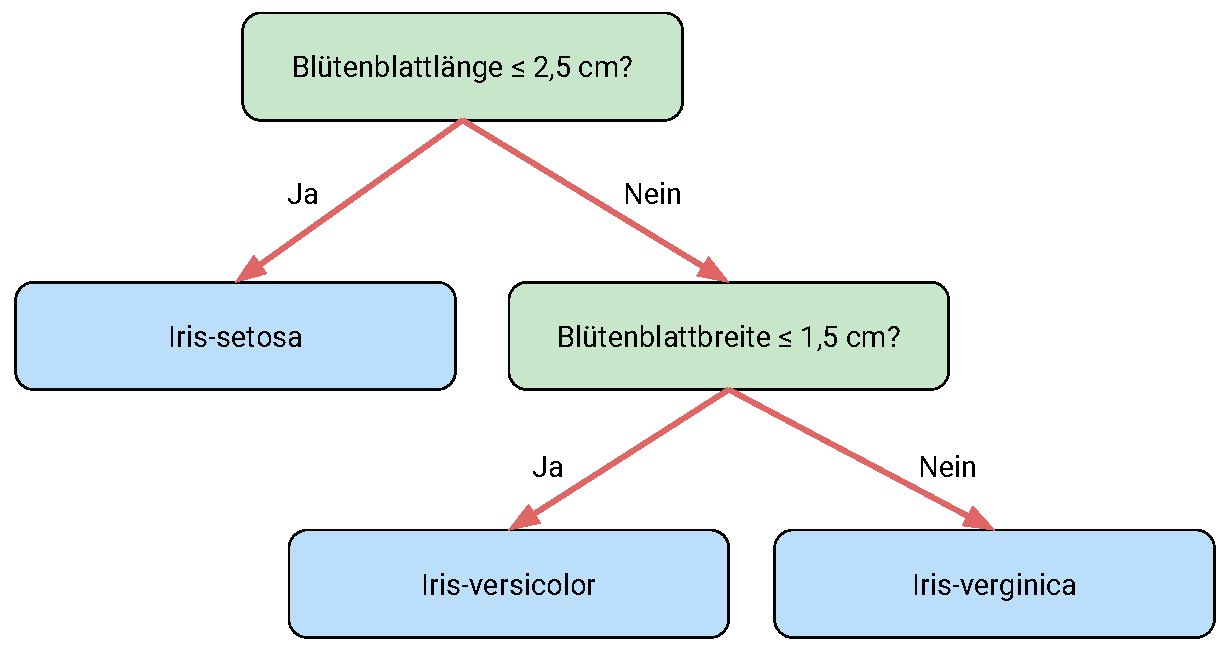
\includegraphics[scale=0.55]{images/kapitel_2/supervised_learning.pdf}
    \caption{Klassifizierung mit einem Ereignisbaumalgorithmus}
    \label{fig:grundlagen_supervised_learning}
\end{figure}

In der Abbildung wird lediglich auf zwei der vier Merkmale eingegangen. Nun ist es möglich auch für die verbleibenden
Kombinationsmöglichkeiten jeweilige Entscheidungsbäume zu erstellen. So entsteht ein sogenannter Random Forest, also ein
Wald von zufälligen Entscheidungsbäumen.

\subsubsection{Unsupervised Learning}
Der k-Means-Algorithmus ist einer der bekanntesten Clustering-Algorithmen im Unsupervised Learning (unüberwachtes
Lernen).

In diesem werden Cluster gesucht, denen Merkmalsträger (Objekte, Fälle) anhand ihrer Merkmale (Inputfaktoren)
zugeordnet werden sollen. Es wird versucht Objekte anhand ihrer Ähnlichkeit zu gruppieren (englisch clustern) (mehr
hierzu unter~\cite{book_grundlagen_learnings})..

Ein Beispiel ist die Gruppierung von Bier anhand der Merkmale Preis, Alkoholgehalt, Stammgewürzgehalt und Schaumstärke.
Die Gruppen werden mithilfe des Algorithmus gesucht und anschließend definiert.

Der Anwender kann lediglich die Anzahl der Cluster definieren, die erstellt werden sollen. Wenn der Anwender k zum
Beispiel mit drei deklariert, werden lediglich drei Cluster aufgebaut, was eine sehr schlechte Unterscheidung zur folge
haben kann.

Die Abblidung~\ref{fig:grundlagen_unsupervised_learning} auf Seite~\pageref{fig:grundlagen_unsupervised_learning} zeigt
die Gruppierung von einzelnen Objekten in drei unabhängige Cluster.

\begin{figure}[h]
    \centering
    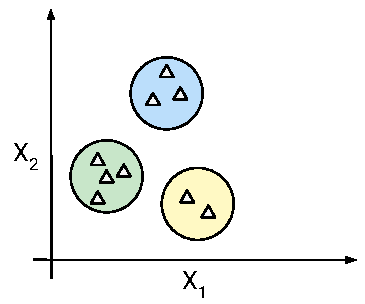
\includegraphics[scale=1.2]{images/kapitel_2/unsupervised_learning.pdf}
    \caption{Clusterbildung beim Unsupervised Learning}
    \label{fig:grundlagen_unsupervised_learning}
\end{figure}

Einer der bekanntesten Einsatzmöglichkeiten für den k-Means-Algorithmus ist die Gruppierung von Kunden anhand
soziodemografischer Merkmale oder Kaufverhalten um ein besseres Bild der eigenen Kundschaft zu erhalten um darauf
aufbauend Maßnahmen definieren zu können.

Damit können zum Beispiel Kundengruppen bessere Werbung geschaltet oder Angebote unterbreitet werden. Auch ausreißer
sind für die Auswertung interessant, da auf diese besser eingegangen werden kann.

Der Algorithmus basiert auf fünf einfachen Schritten die im Weiteren näher erläutert werden. Diese basieren auf der
Anleitung von Golem\footnote{https://bit.ly/2Ev8qNt}.

\begin{itemize}
    \item \textbf{Schritt 1} \\
    Der Anwender wählt die Anzahl der Variablen k. Dies ist die Anzahl der Cluster, welche gebildet werden sollen.
    \item \textbf{Schritt 2} \\
    Wähle k-Punkte als Anfangszentren der Cluster.
    \item \textbf{Schritt 3} \\
    Ordne jeden Punkt, also jeden Merkmalsträger, jenem Zentrum zu, das ihm an nächsten ist. Punkte, die einem Zentrum
    wegen ihrer Nähe zugeordnet wurden, bilden einen Cluster.
    \item \textbf{Schritt 4} \\
    Berechne die k-Clusterzentren neu: Die Zentren sollen sich im Zentrum, also in der Mitte der Cluster, welche in
    Schritt 3 gebildet wurden, befinden.
    \item \textbf{Schritt 5} \\
    Hat sich die Position der Clusterzentren geändert? Wenn ja, springe zu Schritt 3, ansonsten beende das Programm.
\end{itemize}

Dieser Algorithmus ist in zahlreichen Bibliotheken (Libraries) für diverse Programmiersprachen hinterlegt und kann
kostenfrei genutzt werden.

\subsubsection{Reinforcement Learning}
Hinter dem Reinforcement Learning (bestärkendes Lernen) steckt das Prinzip des Trial and Errors verbunden mit einer
Bewertung, die gutes (zielführendes) Verhalten belohnt und schlechte Verhaltensmuster bestraft. Dabei handelt es sich
um selbstständiges lernen indem versucht wird Belohnungen zu maximieren beziehungsweise Strafen zu minimieren.

Der Algorithmus durchläuft viele Iterationen bei denen bewährte Verhaltensmuster miteinander verknüpft werden und neue
ausprobiert werden. Die bekanntesten Algorithmen sind die genetischen Algorithmen, welche sich an der Evolutionstheorie
von Charles Darwin orientieren (mehr dazu unter~\cite{book_grundlagen_learnings}).

Reinforcement Learning kommt bei Lernprozessen zum Einsatz, bei denen auf sich verändernde Umwelteinflüsse reagiert
werden soll. Ein Beispiel ist das trainieren eines Ameisenvolkes zur Suche der optimalen Fortbewegung. Jede einzelne
Ameise würde anfangs irgendwie versuchen sich zu bewegen. Nach und nach würden die einzelnen Ameisen richtiges laufen
aber lernen.

Der messbare Erfolg wäre in diesem Beispiel die zurückgelegte Strecke der einzelnen Ameise. In der nächsten Iteration
würden die erfolgreichsten Fortbewegungstechniken dann miteinander kombiniert und es würde sich ein spürbarer
Fortschritt einstellen.

Die Funktionsweise des Reinforcement Learning ist in Abbildug~\ref{fig:grundlagen_reinforcement_learning} auf
Seite~\pageref{fig:grundlagen_reinforcement_learning} zu sehen.

\begin{figure}[h]
    \centering
    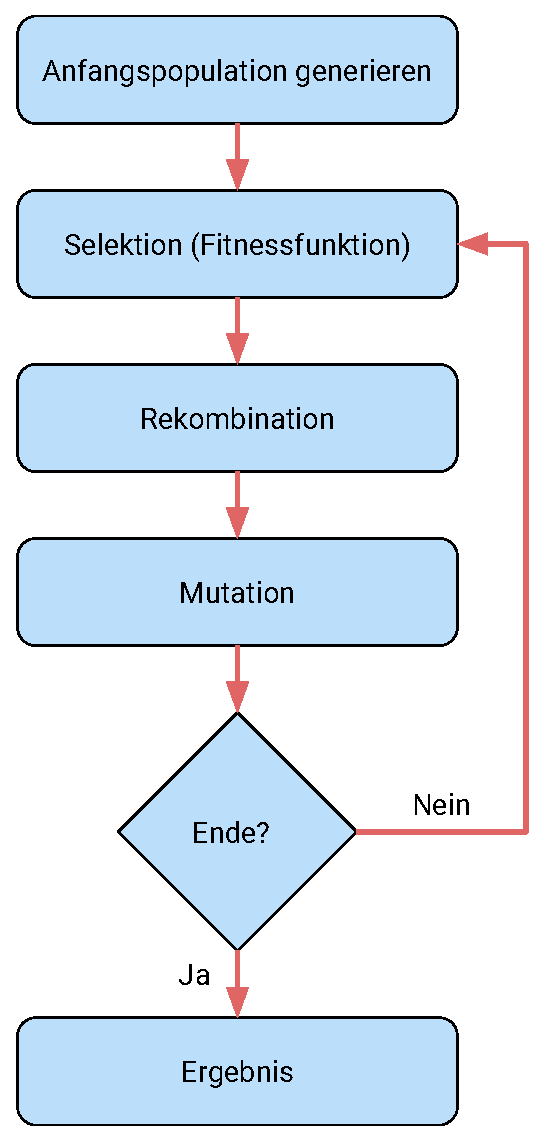
\includegraphics[scale=0.55]{images/kapitel_2/reinforcement_learning.pdf}
    \caption{Funktionsweise des Reinforcement Learnings}
    \label{fig:grundlagen_reinforcement_learning}
\end{figure}

Der Algorithmus endet, sofern entweder das Ziel erreicht beziehungsweise die Zielpunktzahl überschritten wurde. Problem
des bestärkendes Lernens ist es, dass es kein optimales Ergebnis garantiert, sondern lediglich eine Verbesserung von
Generation zu Generation.

Des Weiteren ist das erreichte Ergebnis nicht immer das einzig Mögliche und auch nicht immer wiederholbar. Wenn mit der
gleichen Anfangspopulation gestartet wird, so ist das Ergebnis oft ein anderes, da Rekombinationen und Mutationen durch
Zufall beeinflusst werden.

\subsection{Neuronale Netze}
Bei Neuronale Netze (englisch Neural Network) handelt es sich um Gruppen von Algorithmen die wie ein menschliches Gehirn
aufgebaut sind. Sie sind dafür da, um wiederkehrende Muster zu erkennen und diese daraufhin zu ordnen bzw. zu markieren.

Die erkannten Muster werden anschließend in mathematisch Vektoren übersetzt und alle Informationen der realen Welt wie
Bilder, Sound, Text oder Zeitfolgen berücksichtigt.

Über mehrere Ebenen hinweg helfen neuronale Netze dabei dem jeweiligen System neue Informationen aufgrund von
Ähnlichkeiten zu klassifizieren und in Modellgruppen zusammenzufassen.

Die Labels helfen dabei, die einzelnen Gruppen zu benennen. Für Labels gibt es mehrere Beispiele wie \enquote{Spam},
\enquote{zufriedener Kunde}, \enquote{unzufriedener Kunde}.

Die neuronalen Netzwerke bestehen aus mehreren Ebenen (englisch Layern), die in Reihe geschaltet sind. Sie helfen zur
Verfeinerung der ursprünglichen Annahme (mehr zu neuronalen Netzen unter~\cite{book_grundlagen_neuronalenetze}).

\section{Deep Learning}
Deep Learning könnte als Weiterentwicklung des Machine Learnings bezeichnet werden und ist ein Teilbereich dessen.
Klassische Machine Learning Algorithmen greifen auf feste Modellgruppen zur Erkennung und Klassifizierung zurück. Deep
Learning Algorithmen entwickeln diese Modelle eigenständig weiter oder erstellen neue Modellebenen innerhalb der
neuralen Netzwerke.

Für neue Vorhersagen, neuen Datensätzen oder für neue Tests müssen nicht immer manuell neue Modelle entwickelt und
eingeführt werden, was den Vorgang deutlich beschleuningen kann (mehr über Deep Learning
unter~\cite{book_grundlagen_machinelearning}).

\section{Cloud}
Für Cloud Computing hat sich die Kurzform Cloud etabliert. Dies versteht das Zusammenspiel von mehreren Servern in einem
Verbund. Diese Server übernehmen zum Beispiel Aufgaben wie etwa die Datenspeicherung oder komplizierte Programmabläufe.
Dabei ist für den Cloud-Nutzer nicht ersichtlich, wie viele Server in dieser Cloud stecken oder wo diese sich befinden.

Auch wenn ein Server in diesem Gesamtsystem ausfällt, hat dies keine Auswirkungen auf das gesamte System, da die
Anfragen und Aufgaben auf andere Systeme umgeleitet werden.

Durch NIST~\cite{online_grundlagen_cloud_nist} und~\cite{online_grundlagen_cloud_computing} zeichnet sich die Cloud
durch fünf wesentliche Eigenschaften aus:

\begin{itemize}
    \item \textbf{On-Demand Self Service} \\
    Registrierte Nutzer können Resourcen selbstständig instantiieren und konfigurieren.
    \item \textbf{Broad Network Access} \\
    Der Zugriff kann von verschiedenen Endgeräten erfolgen.
    \item \textbf{Resource Pooling} \\
    Alle Resourcen des Anbieters werden gebündelt und nach Bedarf den Nutzern zugewiesen.
    \item \textbf{Rapid Elasticity} \\
    Kapazitäten können nach Bedarf skaliert werden und stehen schnell und dynamisch zur Verfügung.
    \item \textbf{Measured Service} \\
    Es existiert eine automatische Kontrolle der Ressourcen durch einen Zähler, welcher die Transparenz für den
    Anbieter und den Benutzer ermöglicht.
\end{itemize}

Auf dem Markt existieren zahlreiche Cloud-Anbieter. Im folgenden wird auf drei der Top 10 größten Anbieter und deren
Lösungen im Bereich künstliche Intelligenz eingegangen (siehe hierzu~\cite{online_grundlagen_cloud}).

\subsection{Microsoft Azure}
Azure ist die Cloud-Computing-Plattform von Microsoft. Sie ist hoch skalierbar und wendet sich mit ihren Services
hauptsächlich an Unternehmen und Entwickler. Offiziell ist Azure seit 2010 verfügbar. Seitdem erscheinen in regelmäßigen
Abständen neue Services und Funktionen.

Nutzer der Plattform können Services aus den Bereichen Infrastructure as a Service (IaaS), Platform as a Service (PaaS)
und Software as a Service (SaaS) nutzen. Auch Datenbanken, Storagesysteme sowie virtuelle Maschinen, SQL-Datenbanken und
VPN-Gateways werden bereitgestellt.

Microsoft hat sich mit ihrer Platform Azure das Ziel gesetzt, Anwendern eine flexible Cloud-Infrastruktur zur Verfügung
zu stellen, die sich den individuellen Anforderungen schnell anpassen lässt und den Betrieb einer eigenen IT-Infrastruktur
überflüssig macht.

Dank weltweit betriebener Rechenzentren stehen die Dienste mit einer hohe Verfügbarkeit auf jedem Kontinent zur Verfügung.

Microsoft Azure ermöglicht den Einsatz von Hybrid-Systemen, bei denen nur ein Teil der Services in die Cloud verlagert
und der Rest auf lokalen Servern betrieben wird. Dienste von Drittanbietern bietet ein eigener Azure Marktplatz an
(mehr unter~\cite{online_grundlagen_azure}).

\subsubsection{Azure Machine Learning Studio}
Microsoft Azure Machine Learning Studio ist ein Tool mit dem Vorhersageanalysen erstellt, getestet und bereitgestellt
werden können. Dabei ist es für die Zusammenarbeit mittels Drag \& Drop konzipiert.

Die erstellten Modelle können als Webdiest zur Verfügung gestellt werden. Andere oder auch eigene Anwendungen können
diesen Webdienst mittels HTTP-Anfragen ansprechen und nutzen (siehe dazu~\cite{article_grundlagen_azure_studio}).

\subsection{Amazon Web Services}
AWS ist eine Tochterfirma von Amazon.com und bietet eine umfangreiche Plattform für Cloud-Computing-Services. Genau
wie in Microsoft Azure können dort Services für Infrastucture as a Service (IaaS), Platform as a Service (PaaS) und
Software as a Service (SaaS) genutzt werden.

Im Bereich IaaS haben Nutzer Zugrifff auf Datenspeicherung oder Rechenleistung. Über PaaS haben sie zugriff auf
Services zur einfachen Entwicklung von Webanwendungen. Bei SaaS existiert ein Katalog für Softwareanwendugnen von
externen Dienstleistern.

Ein bekanntes Beispiel für SaaS ist Google Docs, das eine standortunabhängige und Browserunabhängige Bearbeitung von
Dokumenten ermöglicht.

Public Clouds sind für Unternehmen nützlich, um beispielsweise schnell und einfach individuelle Anwendungen entwicklen
zu können ohne notwendige Produktlizenzen anderswo erwerben zu müssen.

AWS stellt Entwicklern eine maßgeschneiderte und zuverlässige IT-Infrastruktur auf Abruf zur Verfügung (= Self Service)
(mehr über AWS unter~\cite{online_grundlagen_aws}).

\subsubsection{Amazon Machine Learning}
Amazon Machine Learning ist ein Service innerhalb von AWS. Es bietet Visualisierungstools und Assistenten die den Aufbau
von Machine Learning-Modellen (ML) unterstützen, ohne dabei komplexe Algorithmen oder Technoligien vorauszusetzen.

Der Service nutzt leistungsstarke Algorithmen um ML-Modelle zu erstellen, indem er in den vorhandenen Daten automatisch
und selbstständig nach Mustern sucht. Anschließend werden diese Modelle dazu genutzt, um neue Daten zu verarbeiten und
Prognosen für eigene Anwendung zu generieren.

Der Service ist hochgradig Skalierbar und kann Milliarden Prognosen pro Tag generieren um diese in Echtzeit mit der
eigenen Anwendung zu teilen (mehr dazu in der Dokumentation~\cite{online_grundlagen_aws_learning}).

Nach dem Aufbau und dem Training der Modelle können diese über eine REST-API anderen Anwendungen zugänglich gemacht
werden, ohne sich dabei selbst um Infrastrukturen kümmern zu müssen.

\subsection{IBM Cloud (ehemals Bluemix)}
Die IBM Cloud (ehemals Bluemix genannt) ist die von IBM entwickelte Cloud Platform. In dieser sind mehr als 160 Services
inbegriffen um zum Beispiel mobile Apps oder Webanwendungen zu entwickeln. Weiter existieren zahlreiche Analysewerkzeuge
sowie Services von Drittanbietern.

Mit Watson Analytics lassen sich beispielsweise intelligente Systeme realisieren, die Daten kognitiv (also selbstlernend,
ohne für die Problemlösungen programmiert zu sein) auswerten und für die Entscheidungsfindung aufbereiten.

Die IBM Cloud unterstützt diverse schon integrierte DevOps-Dienste, um Cloud-Anwendungen zu erstellen, auszuführen,
bereitzustellen und zu verwalten. Die Platform basiert auf der Cloud Foundry Technologie und läuft auf IBMs
Softlayer Infrastruktur.

Sie unterstützt zahlreiche Programmiersprachen, einschließlich Java, Node.js, Go, PHP, Python, Ruby Sinatra, Ruby on
Rails und kann auch andere Sprachen wie Scala durch den Einsatz von Buildpacks unterstützen~\cite{book_grundlagen_bluemix}.

Weitere Informationen über Bluemix finden sich auf der Webseite\footnote{https://bluemix.net} und in der
Dokumentation\footnote{https://eu-gb.dataplatform.ibm.com/docs}.

\subsubsection{Watson Studio}
Watson Studio ist eine SaaS-Lösung der IBM Cloud und für die Erstellung, das Trainieren und das Verwalten von trainierten
Modellen zuständig. Diese Modelle werden, ähnlich denen von Microsoft Azure und AWS, über Drag \& Drop eingerichtet
und Versioniert.

Es bietet eine vielzahl von Anwendungen für die Verarbeitung von Daten und kann mit mehreren Endnutzern gleichzeitig
genutzt werden. In Watson Studio können Modelle erstellt, trainiert und verifiziert werden (mehr hierzu
unter~\cite{online_grundlagen_watson_studio}).

\subsubsection{Cloud Object Storage}
Der Service Cloud Object Storage ist für die Speicherung von unstrukturierten Daten in der Cloud zuständig. Dieser kann
sehr einfach erweitert werden um neuen Bedürfnissen zu genügen.

Die Architektur speichert und managed die Daten über Objekte. Dies hat einen großen Vorteil gegenüber der herkömmlichen
Speicherung über Blöcke und Volumes auf Festplatten. So finden sich alle Informationen, welche einen Datenstamm zugehörig
sind, an einer einzelnen Stelle. Diese Objekte können anschließend sehr einfach kopiert, erweitert oder entfernt werden.

Jedes Objekt hat eine globale und eindeutigen Identifierierung (ID) über die es gefunden werden kann. Außerdem enthält
ein Objekt Metadaten für eine Indezierung (mehr dazu unter~\cite{book_grundlagen_objectstorage}).

\subsubsection{Apache Spark}
Bei Apache Spark handelt es sich um ein Framework, welches unter der Open-Source-Lizenz verfügbar ist. Es ist ein Projekt
der Apache Software Foundation\footnote{https://www.apache.org} und entstand aus einem Forschungsprojekt der University
of California in Berkeley\footnote{https://www.berkeley.edu}.

Apache Spark ermöglicht es, Datenabfragen und große Datenmengen aus unterschiedlichen Quellen in hoher Geschwindigkeit
und guter Performance abzufragen und auszuführen. Dabei wird eine verteilte Architektur und Cluster Computing genutzt.

Viele große Unternehmen unterstützen die Weiterentwicklung von Apache Spark (mehr zu Apache Spark
unter~\cite{book_grundlagen_apachespark}).

\subsubsection{API Connect}
Mit dem Service IBM API Connect können alle vier Aspekte eines Application Programming Interfaces (kurz API)
Lebenszyklusses abgebildet werden: die Erstellung, die Ausführung, das Management und der Schutz einer eigenen API.

Mit diesem Services ist es möglich eine eigene API über ein Drag \& Drop Interface zu definieren und einzurichten. Die
so erstellten Schnittstellen können anschließend einfach über einen Webdienst zur Verfügung gestellt werden.

Dabei ist es möglich, verschienede Routen und Endpunkte zu definieren sowie die Schutzmaßnahmen und eventuelle
Zugangsverwaltung einzurichten (mehr in der Dokumentation~\cite{book_grundlagen_apiconnect}).

\subsubsection{Toolchain}
Bei einer Toolchain handelt es sich um ein Service zur Verwaltung von Entwicklung, Bereitstellung sowie Überwachung
einer Anwendung. Verschiedene Erweiterungen stehen nach der Einrichtung einer Toolchain zur Verfügung.

So ist es anschließend zum Beispiel möglich, eine Integration von einem vorhandenen GitHub-Projekt einzubauen oder eine
Verknüpfung mit einem Slack-Channel einzurichten, welche die wichtigsten Informationen der Toolchain automatisiert teilt.

Nachdem eine eingerichtete Toolchain mit einem Git-Repository verbunden wurde kann der Quelltext gebaut und auf einem
System installiert werden. Das Git-Repository kann entweder auf einem externen Service bereitstehen oder ein IBM internes
GitLab Projekt sein.

Bei der Toolchain handelt es sich unter anderem um ein \textit{Continuous Integration}-Tool (kurz CI)
(mehr über die Toolchain unter~\cite{online_grundlagen_toolchain}).

\section{TensorFlow.js}
TensorFlow ist eine Deep Learning Bibliothek welche von Google entwickelt wird. Die Bibliothek wird unter der freien
Apache 2.0 Lizenz vertrieben und ist sowohl unter allen gängigen Betriebssystemem lauffähig als auch bei den meisten
Cloud-Anbietern. Diese stellen entweder aktuelle Cloud Foundry-Container bereit oder eigene Python-Container.

TensorFlow ist der Nachfolger von Googles erstem Deep Learning Tool \textit{DistBelief}, welcher wiederum aus
\textit{Google Brain} hervorging. Ursprünglich wurde es zur Erkennung von Objekten auf Fotos und Videos entwickelt.

Die Berechnungen von neuronale Netzen können durch TensorFlow auf verteilte Computersysteme geschehen. Dies ist möglich,
da diese intern durch Graphen repräsentiert werden.

Aktuell wird TensorFlow für Predictive Analytics, Fraud Detection oder auch als Recommendation Engine bei Google und
vielen anderen Firmen verwendet.

In der neuesten Version lässt sich TensorFlow ohne großen Aufwand in Python integrieren. Dadurch können neue Lösungen
einfach zur Verfügung gestellt werden (mehr unter~\cite{book_grundlagen_tensorflow}).

Mittlerweile existiert eine mobile Lösung, die TensorFlow.js Bibliothek. Diese ist in jedem gängigen Browser oder auch
in Node.js lauffähig und macht schnelle \enquote{On the Edge}- sowie Offline-Vorhersagen möglich.

\section{Angular}
Bei Angular handelt es sich um ein von Google entwickeltes JavaScript-Framework. Es zielt auf die Entwicklung von
Web-Anwendungen ab und legt großen Wert auf Struktur und Qualität.

Mit seinem großen Fokus auf Architektur, Testing und isolierten Komponenten ist es für große Enterprise Anwendungen
bestens geeignet. Dabei war es das erste JavaScript-Framework das diesen Fokus hatte.

Durch Methoden wie Dependency Injection und ein ausgereiftes Tooling ermöglicht es effiziente und wartbare
Softwareentwicklung auf Basis von JavaScript (mehr unter~\cite{book_grundlagen_angular}).

\subsection{Model-View-Controller}
Die Programmarchitektur Model-View-Controller (kurz MVC) wurde um 1978 von Xerox entwickelt. Dabei wird eine
Anwendungskomponente in drei Teile zerlegt. In das oberflächenunabhängige \textit{Model}, das für die
Ausgabe zuständige \textit{View} und den für die Interpretation von Eingabeereignissen zuständigen \textit{Controller}.

Der Controller ist in dieser Architektur die Steuerungseinheit. Das Model beherbergt den Anwendungskern und die View
die Dargestellten Komponenten auf der Web-App.

Ein Controller zusammen mit einer View wird hier auch als eine Oberfläche bezeichnet. (mehr hierzu
unter~\cite{book_grundlagen_mvc}).

Es gibt zahlreiche Frameworks, welche das MVC-Patern umsetzen. Angular ist einer der bekanntesten Vertreter.

\subsection{Angular-Material}
Material Design ist eine von Google entwickelte Designsprache. Durch diese werden die Gestaltungsregeln des klassischen
Grafik-Designs mit den Möglichkeiten digitaler Benutzeroberflächen verbunden. Ziel ist es unter anderem die Verbesserung
von Benutzeroberflächen zu ermöglichen.

Material Design hat einen charakteristischen Look der es ermöglicht verschiedene Interfaces, welche im Material Design
gehalten sind, einfach zu kombinieren (mehr dazu in~\cite{online_grundlagen_materialdesign}).

Die JavaScript-Library \textit{Angular-Material} ermöglicht eine leichte integration des Material Designs in eine
Angular-Anwendung.

\subsection{ngx-restangular}
Mit der JavaScript-Library ngx-restangular können HTTP-Anfragen an REST-Schnitt\-stellen vereinfacht werden. Dabei
ermöglicht die Library vereinfacht Anfragen mittels den HTTP-Typen \textit{GET}, \textit{POST}, \textit{DELETE} und
\textit{UPDATE} zu stellen (mehr auf der betreffenden GitHub-Seite~\cite{online_grundlagen_restangular}).

Sie unterstützt in der Entwicklung und vereinfacht das Übergeben von Parametern an die Schnittstellen und die
Verarbeitung der Rückgabewerte.

\subsection{Observable}
Ein Observable ist das zentrale Konzept in Reactive Programming mit ReactiveX\footnote{http://reactivex.io}. Es
repräsentiert eine Menge von Daten, die in einer noch nicht bekannten Menge zu einem noch nicht bekannten Zeitpunkt
bereitstehen werden.

Ein Observer abonniert ein Observable und damit die später ankommenden Daten. Diese können gefiltert, gruppiert oder
transformiert werden. Auch Berechnungen sind mit den Daten möglich (mehr unter~\cite{book_grundlagen_observable}).

\subsection{Promise}
Bei Promises handelt es sich um eine Weiterentwicklung von Callbacks. Dabei helfen sie die Arbeit mit asynchronem Code
zu vereinfachen, indem sie asynchrone Operationen kapseln.

Sie zwängen asynchrone Operationen in eine einheitliche API, können verarbeitet werden bevor die Operation abgeschlossen
ist und es gibt zahlreiche Möglichkeiten Promises zu kombinieren oder in Sequenzen zu verwenden (mehr
in~\cite{book_grundlagen_promises} oder unter Matt Greer\footnote{http://www.mattgreer.org/articles/promises-in-wicked-detail}).

\subsection{flex-layout}
Bei flex-layout handelt es sich um ein Angular-Plugin, welches die Flexbox
CSS\footnote{https://www.w3schools.com/css/css3\_flexbox.asp}-Library für Angular implementiert.

Das Plugin hilft dabei, Webseiten auf verschiedene Browsergegebenheiten anzupassen. Dazu zählt unter anderem die Größe
des Displays oder die verwendete Version des Browsers.

Das Plugin hilft bei der Erstelltung von responsiven Webseiten indem es verschiedene Breakpoints zur Verfügung stellt
(mehr auf der GitHub-Page~\cite{online_grundlagen_flexlayout}).

\section{REST}
Representational State Transfer - Application Programming Interface (kurz REST-API) macht den Austausch von Informationen
über unterschiedliche Systeme möglich. Im Zeitalter verteilter Systeme und Cloud-Computing ist der Einsatz von REST-APIs
zur Kommunikation zwischen den Systemen notwendig.

Auch spricht man bei REST-APIs von Maschine-Maschine-Kommunikation, da die verschiedenen Systeme so eine gemeinsame
Sprache sprechen können um sich zu verständigen.

Mit der Hilfe von REST-APIs ist es möglich geworden, Informationen und Aufgaben auf verschiedene Systeme zu verteilen
(Microservices). Mit HTTP-Requests können Informationen dann verteilt werden. Jeder HTTP-Request setzt sich aus dem
Endpoint und den entsprechenden Parametern zusammen~\cite{online_grundlagen_rest}.

\section{Cloud Foundry}
Cloud Foundry ist eine Open Source Platform as a Service Lösung. Damit ist es für Entwickler möglich Anwendung zu bauen,
hochzuladen und auszuführen. Die nahezu grenzenlose Skalierbarkeit ist einer der größten Vorteile von Cloud
Foundry~\cite{book_grundlagen_cloudfoundry}.

Diese Skalierbarkeit wird durch die Container-Architektur erreicht. Jeder Container beinhaltet eine eigene
Anwendungsinstanz. Cloud Foundry unterstützt sowohl eine horizontale als auch eine vertikale Skalierung.

Bei der horizontalen Skalierung werden zusätzliche Container gestartet oder gestoppt. Ein Load Balancer kümmert sich um
die Verteiltung des Traffics. Bei der vertikalen Skalierung werden jeder Instanz individuell z.B. mehr oder weniger
Arbeitsspeicher oder CPU Zeit zugeteilt.

In der IBM Cloud erhält jede Cloud Foundry Instanz eine eigene IPV4-Adresse wodurch es mittels A-Record (Zuordnung eines
DNS-Namens zu IP-Adresse) möglich ist, eine eigene Domain mit der Anwendung zu verknüpfen.

\section{Version Control (Git)}
Git ist ein verteiltes Versionierungssystem, dass frei als Open-Source-Software zur Verfügung steht. Es wird bei der
Softwareentwicklung für die Versionskontrolle (stetige Protokollierung von Änderungen) von Dateien eingesetzt. (mehr
unter~\cite{book_grundlagen_git}).

\section{Node Package Manager (npm)}
Der Node Package Manager (kurz npm) ist ein Paketmanager für Node.js. Mit diesem lassen sich unter anderem
Software-Pakete für die Entwicklung von Projekten verwalten und steuern.

Es existiert eine Sammlung von Paketen (Repository) auf der offiziellen Webseite\footnote{https://www.npmjs.com}. Über
den entsprechenden Namen lassen sich die Pakete finden und im eigenen Projekt verwenden
(mehr unter~\cite{book_grundlagen_npm}).

\section{Mockups}
Ein Mockup findet seinen Einsatz bei der Planung von Webauftritten oder sonstigen Softwareprojekten welche eine grafische
Ausgabe besitzen. Mit diesen ist es möglich einen ersten Eindruck von der Gestaltung und den Funktionalitäten der
Anwendung zu bekommen. Ein großer Vorteil bei der Entwicklung von Mockups ist die Tatsache, dass kein Quellcode dafür
notwendig ist.

Mockups können auf dem Papier oder auch Computergestützt mit zahlreichen Programmen erstellt werden. Dazu zählt zum
Beispiel Balsamiq Mockups\footnote{https://balsamiq.com}.

Bei einem Mockup geht es darum, die verschiedenen Elemente einer Anwendung anzuordnen und einen optimalen Userflow
zu relaisieren. Das Design und etwaige Farben treten in den Hintergrund (mehr unter~\cite{book_grundlagen_mockups}).

\section{TypeScript}
Bei TypeScript (kurz TS) handelt es sich um ein Superset von JavaScript. Dies bedeutet, dass TypeScript ebenfalls eine
Implementierung von ECMAScript\footnote{https://en.wikipedia.org/wiki/ECMAScript} ist, JavaScript jedoch um zusätzliche
Features erweitert.

Jeder geschriebene JavaScript-Code funktioniert auch in TypeScript. Allerdings funktioniert nicht jeder TypeScript-Code
in JavaScript.

TypeScript erweitert JavaScript um mehrere Typings (und Annotations). Dies bedeutet, dass TypeScript, genau wie zum
Beispiel Java, Typensicher ist (mehr dazu unter~\cite{book_grundlagen_typescript}).

Im Listing~\ref{ls:grundlagen_typescript} auf Seite~\pageref{ls:grundlagen_typescript} ist ein originaler
JavaScript-Code in Zeile 2 zu sehen. In der Zeile 5 steht der entsprechende TypeScript-Code. Hier ist die
Typensicherheit gut zu erkennen.

\begin{lstlisting}[language=JavaScript, caption=Unterschied zwischen JavaScript und TypeScript, label=ls:grundlagen_typescript]
    // JavaScript
    var name = "Vorname Nachname";

    // TypeScript
    let name : string = "Vorname Nachname";
\end{lstlisting}

\section{WebView}
Ein WebView ist ein Android- oder iOS-Layout, welches Webseiten darstellen kann. Über diverse Schnittstellen werden dem
Layout Informationen wie Domain, Titel oder Größe übergeben. Das Layout kümmert sich anschließend selbstständig um das
Laden der entsprechenden Webseite und die Darstellung auf dem Bildschirm.

Das Layout steht sowohl unter Android als auch unter iOS seit den frühesten Versionen zur Verfügung (weitere
Informationen unter~\cite{online_grundlagen_webview}).